% chapter 5: efficacy of dose painting on uncertain radiobiological tumor maps
The biological model deployed in this novel approach to dose painting encompasses four different parameters. While the $I_\mathrm{max}$ is a parameter that is dependent on the tracer (here FMISO) and has to be adapted to clinical oxygen values from direct Eppendorf measurements. A robustness analysis was performed for biological dose painting to assess the impact of model uncertainties. For this, the approved biological dose painted plan on the mean model parameters was used to evaluate changes of biological effect on new tumour maps derived from model parameter combinations. Three parameters were evaluated within their standard deviation, which means that every parameters had a lower limit (mean - standard deviation), mean and upper limit (mean + standard deviation). Therefore, $3^3=27$ plans have to be evaluated by comparing the eDVH distributions and their impact on the delivered effect from their underlying HRF distributions. 
\section{Model parameter uncertainties}
This work will investigate all parameters involved in the calculation of dose escalation factors in hypoxic sub volumes. The theoretical implications of the errors on the model parameters $p_{50}$, $K$ and $m$ are shown in figure \ref{fig:uncertaintyimpact}. The largest deviation in HRF transformation is given by the $p_{50}$ parameters, while $m$ and $K$ have a smaller impact. 
\begin{figure}[p]
\centering
\subfigure[$K=1.81$ mmHg, $m=2.77$]{
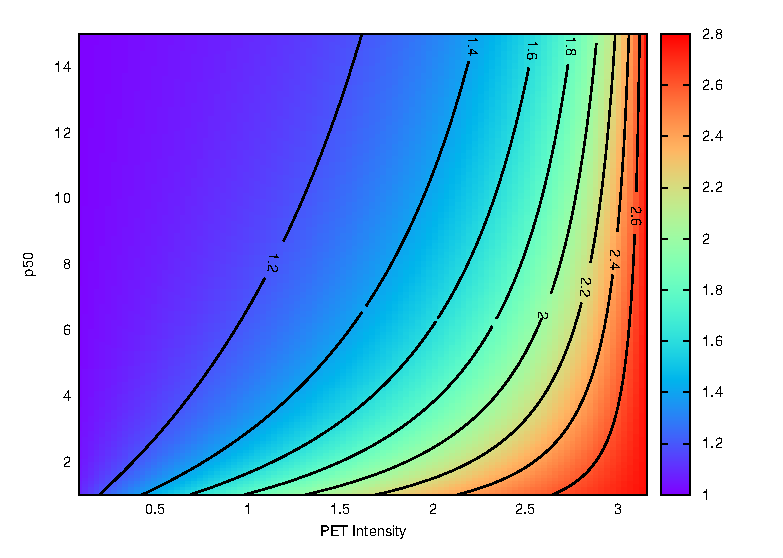
\includegraphics[scale = 0.525]{/Users/alex/Master/contents/images/K181m277.eps}
}
\hspace{0.3cm}
\subfigure[$K=2.07$ mmHg, $m=2.87$]{
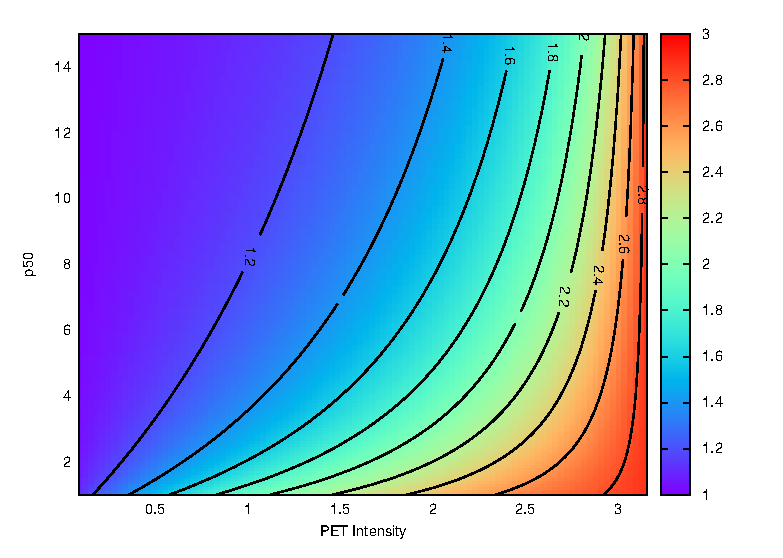
\includegraphics[scale = 0.525]{/Users/alex/Master/contents/images/K207m287.eps}
}
\hspace{0.3cm}
\subfigure[$K=1.81$ mmHg, $p_{50}=1$ mmHg]{
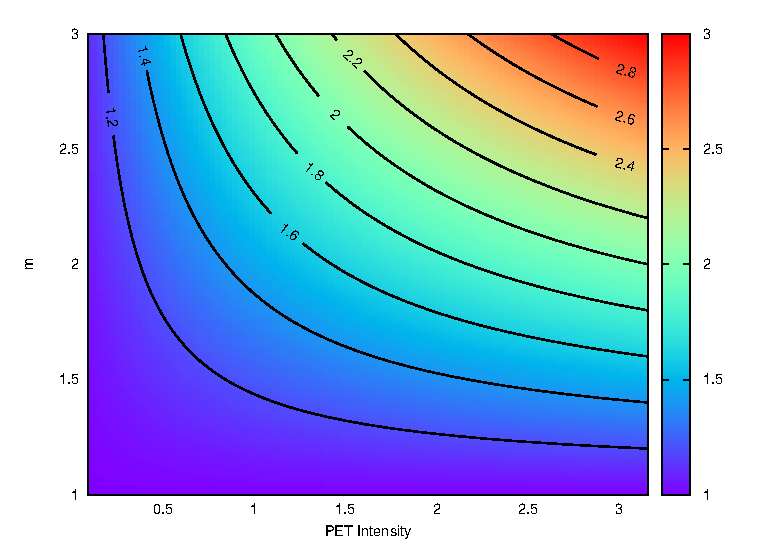
\includegraphics[scale = 0.525]{/Users/alex/Master/contents/images/K181p1.eps}
}
\hspace{0.3cm}
\subfigure[$K=2.07$ mmHg, $p_{50}=11.8$ mmHg]{
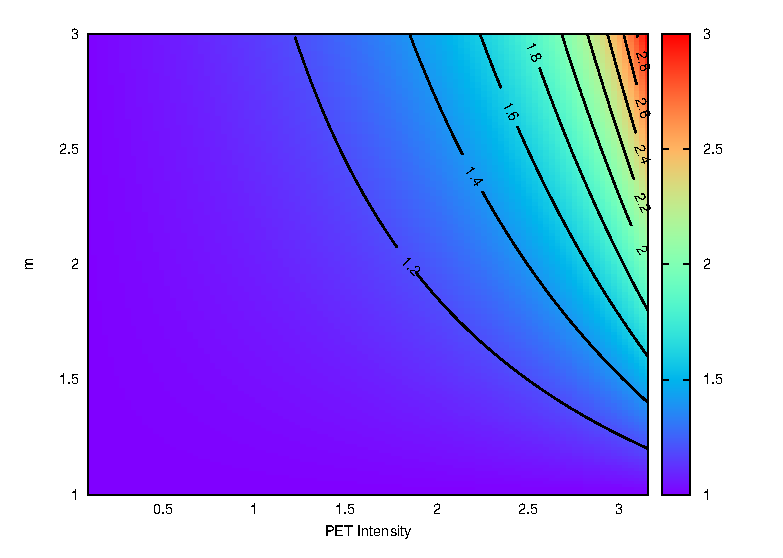
\includegraphics[scale = 0.525]{/Users/alex/Master/contents/images/K207p118.eps}
}
\subfigure[$m=2.77$ mmHg, $p_{50}=11.8$ mmHg]{
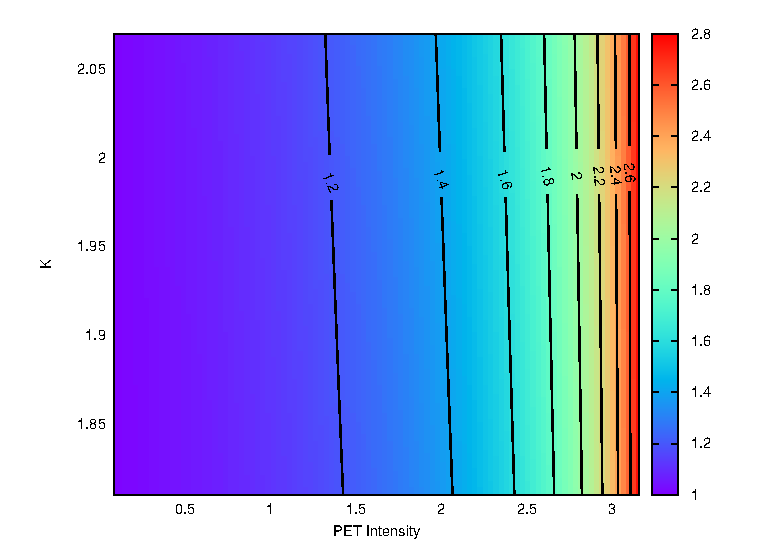
\includegraphics[scale = 0.525]{/Users/alex/Master/contents/images/m277p118.eps}
}
\hspace{0.3cm}
\subfigure[$m=2.87$ mmHg, $p_{50}=1$ mmHg]{
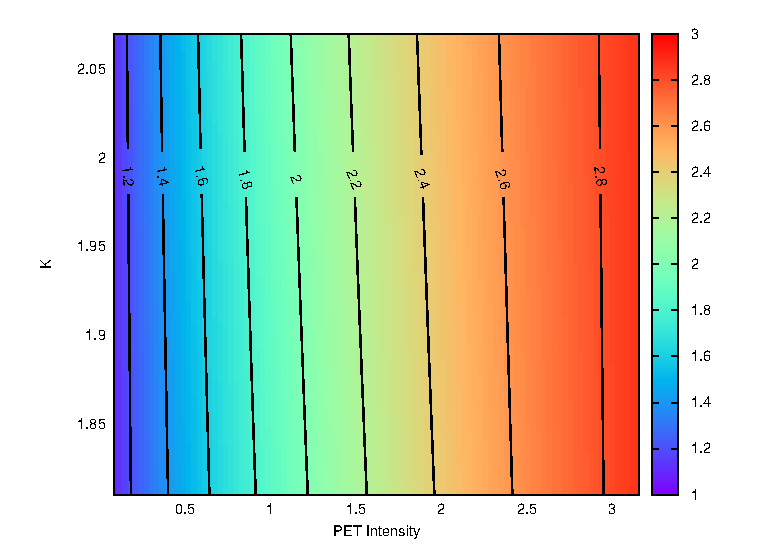
\includegraphics[scale = 0.525]{/Users/alex/Master/contents/images/m287p1.eps}
}
\caption{Impact of model uncertainties on the HRF derived from the signal of a PET FMISO image in the SUV range of 0 up to 3.17. The lowest impact on the HRF prescriptions is seen with $K$, while $p_{50}$ and $m$ introduces the largest HRF changes in the transformation model.}
\label{fig:uncertaintyimpact}
\end{figure}
\subsection{pO2 model}
The pO2 model from \textit{Chang et al.} uses two parameters. The $I_\mathrm{max}$ parameters is a parameters, which can be adjusted to the latest pO2 measurements in any cancer geometry for a specific tracer. For head and neck cancer with FMISO, this value has been calculated to be $I_\mathrm{max}=3.17$. The other parameter is the $p_{50}$ value, which represents the pO2 value where the PET intensity is $I_\mathrm{max}/2$. This value has been measured by \textit{Chang et al.} with a large error
\begin{equation}
p_\mathrm{50} = 6.4 \pm 5.4 \mathrm{mmHg}.
\end{equation}
As the error on this parameters is about 85\% of the original value, it has a larger impact on these values in the theoretical framework that is relevant for the the calculation of HRF. This has direct implications on the delivered effect as the $p_{50}$ parameter governs the range of how PET intensities are interpreted as pO2 values.
\paragraph{Lower limit ($\mathbf{p_{50}=1}$ mmHg)}The $p_{50}$ is interpreted as the oxygen partial pressure, where the PET intensity is $I_\mathrm{max}/2\approx 1.59$. Therefore if the PET SUV is lower, the pO2 will be lower than 1 mmHg. The HRF in these voxels is then close to its maximum value, as the peak HRF is reached at 0 mmHg. Together with the mean parameter values $m=2.82$ and $K=1.94$, the HRF for 1 mmHg is HRF=2.2. Therefore, dose escalations based on a initial 70 Gy prescription are then $D=154$ Gy.
\paragraph{Mean ($\mathbf{p_{50}=6.4}$ mmHg)}The HRF changes dramatically to HRF=1.42, as the $K=1.94$ value plays a big role in the HRF transformation. The largest change in HRF is seen, as soon as the $p_{50}$ value is larger than the $K$ value. This is because, the HRF transformation function has sigmoidal shape and $K$ is the threshold parameter. The dose boost based on a 70 Gy prescription is 99.4 Gy.
\paragraph{Upper limit ($\mathbf{p_{50}=11.8}$ mmHg)}Here the HRF changes slightly to HRF=1.26 as the transformation function for HRF slowly reaches its plateau. By construction, the larger the pO2 values derived from the oxygen model, the lower the HRF. However, mathematically even muscle tissue (40 mmHg) exhibits HRF=1.08. This could imply, that the parameterization of the oxygen model deployed in this approach could be gauged with another parameter (cf. chapter \ref{}). The dose escalation based on a 70 Gy prescription is then 88.2 Gy.
\subsection{Hypoxia reduction factors}
HRFs are dependent on two parameters. The $m$ value as the maximum HRF value and $K$, which is the oxygen partial pressure at $m/2$. While $m$ is a general scale for the HRF within a volume, the $K$ value poses as a threshold value. In contrast to the pO2 model, all parameters deployed in the HRF model exhibit small errors. The $K$ value shows an error of 1.7\%, while $m$ has an error of 6.7\%. Therefore, the range of HRF caused by uncertainties is much smaller, than with the pO2 model.
\section{Results}
Due to the fact, that the pO2 model directly interprets the PET intensity as oxygen partial pressures, it has direct implications on how the HRF transformation function computes HRF and their corresponding dose escalations in the biological optimization. As the $p_{50}$ value approaches 1 mmHg, most voxels are seen as highly hypoxic, which implies high HRF values. Figure \ref{fig:eDVHRobust} shows the eDVH for all 27 plans (for patient 1), as well as the clinical and delivered plan for a representative patient. All eDVH curves are evaluated based on the dose painted plan with mean values. The previously discussed impact of $p_{50}$ can be clearly seen by the clustering of eDVH lines around the 1 mmHg, 6.4 mmHg and 11.8 mmHg parameter values. The differentiation between both HRF transformation parameters $K$ and $m$ is marginally small. Nevertheless, small differences can be seen. The larger the K value, the more voxels are shifted to a larger HRF giving them a high radioresistance. As $m$ is general scale for the HRF, a larger $m$ value will stretch the HRF range, while smaller $m$ parameters will bulge it. The different HRF generated from the model parameters therefore lead to an over and underestimation on the HRF values as well as the current oxygen partial pressure.\\Generally speaking, planning robustness suffers from the large error on $p_{50}$, while $K$ and $m$ have small impact on the overall HRF distribution. The latter is due to the fact, that the errors to $m$ and $K$ are lower than 10\%, while the error on $p_{50}$ is eight times larger. Likewise, the pO2 prescription model has a larger range of values, as oxygen partial pressures are usually found between 0 mmHg and 40 mmHg (and more) in a usual patient. Therefore, errors in this function have implications in term of value range.
\begin{figure}[htb]
\centering
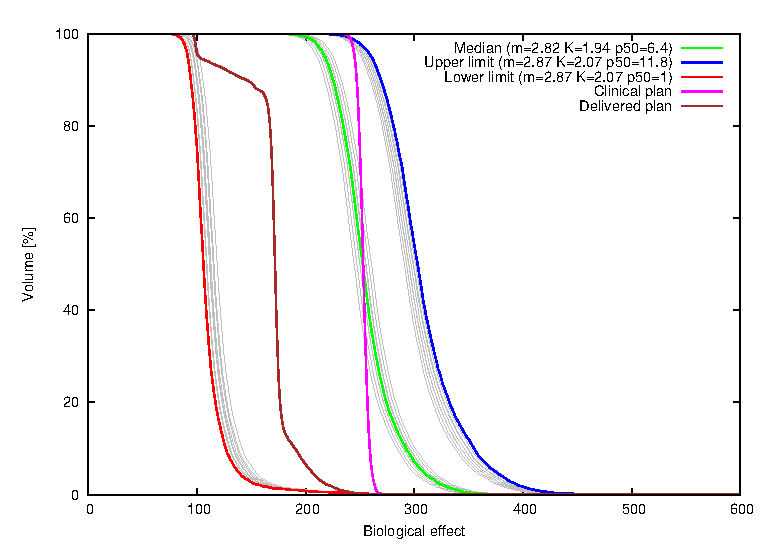
\includegraphics[scale = 1.2]{/Users/alex/Master/contents/images/eDVHRobust.eps}
\vspace{1cm}
\caption{Impact of model parameters uncertainties on the eDVH for patient 1 based on the approved biological dose painted plan with mean values for $K$, $m$ and $p_{50}$.}
\label{fig:eDVHRobust}
\end{figure}
\section{Discussion}
When evaluated with uncertainties, the deployed model shows large differences in HRF distributions, which then lead to different hypoxia tumour maps. In comparison to the tumour map from the plan with mean parameter values, these maps represent scenarios, where the ignorance toward model uncertainties create an over or under estimation of oxygen partial pressures. If the tumour map derived from mean model parameters over estimates the HRF, then dose escalations are set too high in the optimization leading to bad treatment plans. On the other hand, if the mean plan underestimated oxygen partial pressures, dose escalations will not reach the level that is needed to achieve the anticipated biological effect. However, it should be pointed out, that in both cases (over and underestimation of HRF) do not lead to a worse treatment plan than the clinical plan. This is due the fact, that the HRF values can never be lower than 1. Therefore, dose painting can only increase tumour control probability as it only increases (and never decreases) the dose value in a voxel based on the hypoxia map.\\The largest impact on the HRF distributions is due to the large error on the $p_{50}$ parameter from the pO2 model derived by \textit{Chang et al.} as it has a big impact on the range of pO2 value extrapolated from the PET FMISO image. As the $m$ and $K$ parameters only show a small error, which 8 times smaller than the one on $p_{50}$. Therefore it would be desirable to obtain a better measurement on this parameter. 
\section{Conclusion}
The model used in this thesis for the calculation of dose escalations based on FMISO PET images lacks clear robustness as the error on the $p_{50}$ parameter of the pO2 model from \textit{Chang et al.}\ref{pmid19994538} is extremely large. This leads to a wide range of possible HRF distributions that determine the dose escalations in hypoxic volumes. Other sophisticated pO2 models or a better measurement of the $p_{50}$ value would increase the robustness of biological dose painting. However biological dose painting does not create plans that are worse than the clinical plan, as the HRF is limited to values larger than 1.